\documentclass[11pt,twocolumn]{article}

% ── Page layout ──────────────────────────────────────────
\usepackage[margin=0.85in,top=1in,bottom=1in]{geometry}
\usepackage{microtype}

% ── Tables ───────────────────────────────────────────────
\usepackage{booktabs}
\usepackage{multirow}

% ── Charts ───────────────────────────────────────────────
\usepackage{pgfplots}
\usepackage{pgfplotstable}
\pgfplotsset{compat=1.18}

% ── Colors ───────────────────────────────────────────────
\usepackage[table]{xcolor}
\definecolor{controlblue}{HTML}{4472C4}
\definecolor{wikiorange}{HTML}{ED7D31}
\definecolor{hcA}{HTML}{1a9850}   % >= 0.90
\definecolor{hcB}{HTML}{91cf60}   % 0.80 -- 0.89
\definecolor{hcC}{HTML}{fee08b}   % 0.70 -- 0.79
\definecolor{hcD}{HTML}{fc8d59}   % 0.50 -- 0.69
\definecolor{hcE}{HTML}{d73027}   % < 0.50

% ── Heatmap cell command ─────────────────────────────────
\newcommand{\hc}[1]{%
  \ifdim#1pt>0.895pt\relax\cellcolor{hcA!30}%
  \else\ifdim#1pt>0.795pt\relax\cellcolor{hcB!40}%
  \else\ifdim#1pt>0.695pt\relax\cellcolor{hcC!60}%
  \else\ifdim#1pt>0.495pt\relax\cellcolor{hcD!50}%
  \else\cellcolor{hcE!50}%
  \fi\fi\fi\fi%
  #1%
}

% ── Links ────────────────────────────────────────────────
\usepackage[
  colorlinks=true,
  linkcolor=blue!60!black,
  citecolor=blue!60!black,
  urlcolor=blue!60!black
]{hyperref}

% ── Compact sections ─────────────────────────────────────
\usepackage{titlesec}
\titlespacing*{\section}{0pt}{10pt}{4pt}
\titlespacing*{\subsection}{0pt}{6pt}{2pt}

% ── Subfigures ───────────────────────────────────────────
\usepackage{subcaption}

% ── Float control ──────────────────────────────────────────
\usepackage{float}
\usepackage{placeins}
\usepackage{flushend}

% ── Compact lists ────────────────────────────────────────
\usepackage{enumitem}
\setlist{nosep,leftmargin=*}

% ═════════════════════════════════════════════════════════
\title{Does Wikipedia Make Code Better?\\A Load Balancer Case Study}
\author{Timothy Brinded}
\date{February 2026}

\begin{document}
\maketitle

% ─────────────────────────────────────────────────────────
% ABSTRACT
% ─────────────────────────────────────────────────────────
\begin{abstract}
We test whether augmenting an LLM coding agent with access to Wikipedia
improves the quality of generated code.  A single design-rich programming
problem---a graceful-degradation load balancer---is implemented by Claude
Code under eight conditions: one control and seven Wikipedia-augmented
variants with different research strategies.  Solutions are evaluated by
three complementary methods: a blinded LLM judge (design quality), a
deterministic behavioral benchmark (7 fault scenarios, weighted 0--100),
and quantitative cost metrics.  The adversarial \textit{contrarian}
condition, which stress-tests the obvious approach before coding, achieves
the highest benchmark score (92.9 vs.\ 84.7 control).  Architectural
ambition can hurt: the \textit{consilience} condition builds the most
sophisticated design but scores last on benchmarks (76.2).  Judge and
benchmark rankings diverge meaningfully, suggesting each captures
different dimensions of code quality.
\end{abstract}

% ─────────────────────────────────────────────────────────
% 1. INTRODUCTION
% ─────────────────────────────────────────────────────────
\section{Introduction}

Large language models generate competent code from training data alone.
But can cross-domain knowledge---the kind found in encyclopedic
references---improve the \emph{design} of generated software?  We test a
simple hypothesis: giving a coding agent access to Wikipedia articles
alongside a programming problem produces better-designed code than coding
without external references.

We study a single problem: implementing a load balancer with graceful
degradation.  Load balancers are design-rich systems where multiple valid
architectures exist, failure modes are subtle, and cross-domain analogies
(TCP congestion control, biological homeostasis, power grid protection)
can yield structural insights.

Eight conditions are evaluated.  The \textbf{control} receives only the
problem specification.  Seven Wikipedia-augmented conditions each use a
different research strategy: direct research (\textit{explicit}), ambient
exposure (\textit{subtle}), historical precedent (\textit{reflective}),
undirected exploration (\textit{flaneur}), cross-domain convergence
(\textit{consilience}), biological analogy (\textit{biomimetic}), and
adversarial critique (\textit{contrarian}).
Table~\ref{tab:conditions} summarizes all eight conditions.

\begin{table}[ht]
\centering\small
\caption{Experimental conditions and research strategies.}
\label{tab:conditions}
\begin{tabular}{@{}lp{4.6cm}@{}}
\toprule
\textbf{Condition} & \textbf{Research Strategy} \\
\midrule
control     & No Wikipedia access \\
explicit    & Instructed to research Wikipedia \\
subtle      & Wikipedia tools available, not mentioned \\
reflective  & Seek historical precedent and past failures \\
flaneur     & Undirected random Wikipedia exploration \\
consilience & Find convergent patterns across 5+ domains \\
biomimetic  & Research only biological analogies \\
contrarian  & Stress-test the obvious approach first \\
\bottomrule
\end{tabular}
\end{table}

% ─────────────────────────────────────────────────────────
% 2. METHOD
% ─────────────────────────────────────────────────────────
\section{Method}

\subsection{Experimental Setup}

Each condition runs Claude Code in non-interactive mode
(\texttt{claude~-p}) with an identical problem specification.  The agent
implements an \texttt{AbstractLoadBalancer} base class with four required
methods: \texttt{on\_backend\_added}, \texttt{route\_request},
\texttt{on\_request\_complete}, and \texttt{on\_tick}.  Backend health is
inferred through an opaque \texttt{BackendHandle} protocol---the agent
cannot query health directly, only observe request outcomes and probe
results.  Each Wikipedia condition's research agent explores the local
corpus with the same tools it uses for code---ripgrep for cross-article
full-text search, file reads for deep inspection---treating the
encyclopedia as a searchable corpus rather than a lookup API.

\subsection{Conditions}

The \textbf{control} receives the problem specification and nothing else.
All seven Wikipedia conditions receive the same specification plus a
Wikipedia research agent (\texttt{wiki-explorer}) with access to
${\sim}$7 million local Wikipedia articles.  The conditions differ only in
their system prompt framing:

\begin{itemize}
\item \textbf{Explicit}: ``Research Wikipedia for load balancer design
      patterns.''
\item \textbf{Subtle}: Tools available silently; no mention in prompt.
\item \textbf{Reflective}: ``Find historical failures that inform
      resilient design.''
\item \textbf{Flaneur}: ``Take a random walk through Wikipedia; let
      connections emerge.''
\item \textbf{Consilience}: ``Find the same pattern in 5+ unrelated
      domains.''
\item \textbf{Biomimetic}: ``Research only biological systems as design
      analogies.''
\item \textbf{Contrarian}: ``Before coding, find reasons the obvious
      approach fails.''
\end{itemize}

\subsection{Evaluation}

Solutions are evaluated by three independent methods.

\textbf{Deterministic Benchmark.}  Seven fault-injection scenarios run
against each implementation, producing scores on $[0,1]$ per scenario.  An
aggregate score is computed as the weighted average scaled to $[0,100]$.

\textbf{Blinded LLM Judge.}  Each Wikipedia condition is paired against
control in a blinded A/B comparison (randomized assignment to ``Solution
A'' and ``Solution B'').  The judge scores six dimensions: correctness
($\times3$), design ($\times2$), robustness ($\times2$), algorithmic
novelty ($\times2$), cross-domain insight ($\times1$), and
proportionality ($\times1$).  Maximum weighted total: 110 points.

\textbf{Quantitative Metrics.}  Duration, API cost, lines of code, and
subagent token usage are recorded for each run.

\subsection{Benchmark Design}

Table~\ref{tab:scenarios} lists the seven benchmark scenarios and their
weights.  Priority Protection carries the highest weight (3.0) because
correctly shedding low-priority traffic during overload is the core
requirement.  Degradation Detection (2.0) tests whether the agent can
sense a backend that is slowly failing---a subtle scenario that separates
sophisticated health tracking from naive approaches.

\begin{table}[ht]
\centering\small
\caption{Benchmark scenarios and weights.}
\label{tab:scenarios}
\begin{tabular}{@{}lp{3.2cm}c@{}}
\toprule
\textbf{Scenario} & \textbf{Tests} & \textbf{Weight} \\
\midrule
Steady State  & Even distribution, full success   & 1.0 \\
Degradation   & Detect slowly failing backend     & 2.0 \\
Priority      & Shed low-priority traffic first   & 3.0 \\
Recovery      & Smooth ramp-up after failure       & 2.0 \\
Cascading     & Isolate failure, protect healthy   & 2.0 \\
Flapping      & Handle on/off oscillation          & 1.5 \\
Asymmetric    & Route by backend speed             & 1.0 \\
\bottomrule
\end{tabular}
\end{table}

% ─────────────────────────────────────────────────────────
% 3. RESULTS
% ─────────────────────────────────────────────────────────
\section{Results}

\subsection{Benchmark Rankings}

Figure~\ref{fig:benchmark} shows aggregate benchmark scores ranked by
performance.  The \textit{contrarian} condition achieves the highest score
(92.9), outperforming control (84.7) by $+8.2$ points.  Six of seven
Wikipedia conditions outperform control.  The lone exception is
\textit{consilience}~(76.2), which ranks last despite building the most
architecturally ambitious solution.

\begin{figure*}[t]
\centering
\begin{minipage}[t]{0.48\textwidth}
\centering
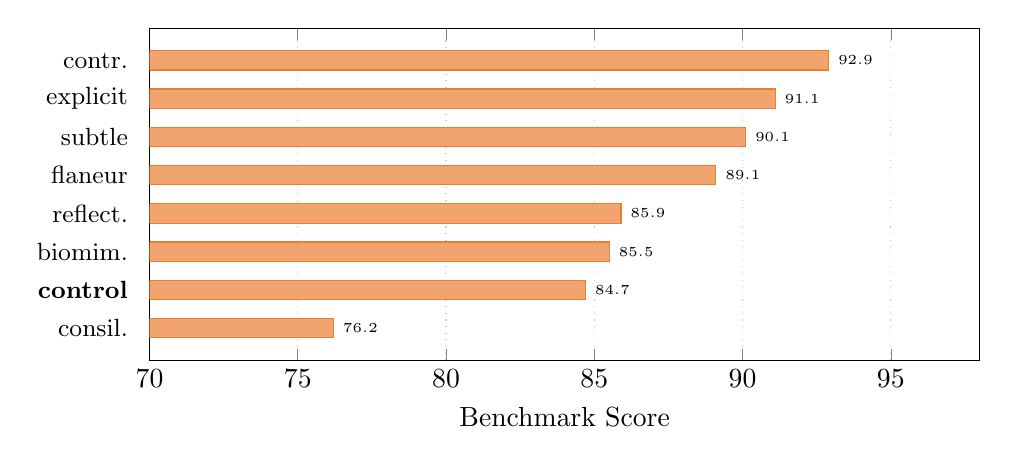
\begin{tikzpicture}
\begin{axis}[
    xbar,
    width=\textwidth,
    height=5.8cm,
    xlabel={Benchmark Score},
    xmin=70, xmax=98,
    symbolic y coords={%
      consil.,control,biomim.,reflect.,%
      flaneur,subtle,explicit,contr.},
    ytick={consil.,control,biomim.,reflect.,%
      flaneur,subtle,explicit,contr.},
    yticklabels={consil.,\textbf{control},biomim.,reflect.,%
      flaneur,subtle,explicit,contr.},
    yticklabel style={font=\small},
    ytick style={draw=none},
    bar width=7pt,
    enlarge y limits=0.12,
    xmajorgrids=true,
    grid style={dotted,gray!40},
    nodes near coords,
    nodes near coords align={horizontal},
    every node near coord/.append style={font=\tiny},
]
\addplot[fill=wikiorange!70, draw=wikiorange]
  coordinates {
    (76.2,consil.)
    (84.7,control)
    (85.5,biomim.)
    (85.9,reflect.)
    (89.1,flaneur)
    (90.1,subtle)
    (91.1,explicit)
    (92.9,contr.)
  };
\end{axis}
\end{tikzpicture}
\subcaption{Aggregate benchmark scores (0--100).  Control baseline in bold.}
\label{fig:benchmark}
\end{minipage}%
\hfill%
\begin{minipage}[t]{0.48\textwidth}
\centering
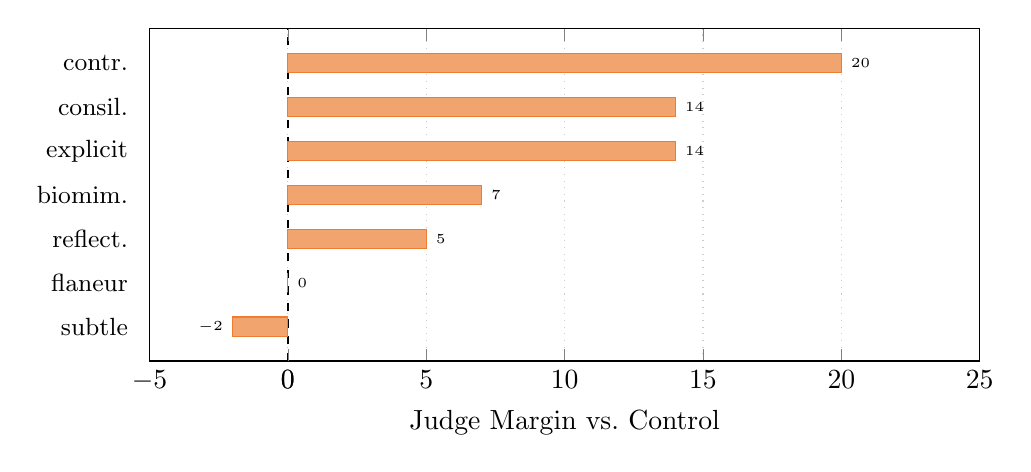
\begin{tikzpicture}
\begin{axis}[
    xbar,
    width=\textwidth,
    height=5.8cm,
    xlabel={Judge Margin vs.\ Control},
    xmin=-5, xmax=25,
    symbolic y coords={%
      subtle,flaneur,reflect.,biomim.,%
      explicit,consil.,contr.},
    ytick=data,
    yticklabel style={font=\small},
    ytick style={draw=none},
    bar width=7pt,
    enlarge y limits=0.13,
    xmajorgrids=true,
    grid style={dotted,gray!40},
    nodes near coords,
    nodes near coords align={horizontal},
    every node near coord/.append style={font=\tiny},
    extra x ticks={0},
    extra x tick style={grid=major, grid style={black,thick,dashed}},
]
\addplot[fill=wikiorange!70, draw=wikiorange]
  coordinates {
    (-2,subtle)
    (0,flaneur)
    (5,reflect.)
    (7,biomim.)
    (14,explicit)
    (14,consil.)
    (20,contr.)
  };
\end{axis}
\end{tikzpicture}
\subcaption{Blinded LLM judge margin vs.\ control (out of 110).
Positive = Wikipedia wins.}
\label{fig:judge}
\end{minipage}
\caption{Benchmark scores (left) and judge margins (right).  Six of seven
Wikipedia conditions beat control on both measures, though the rankings
diverge substantially (see Section~\ref{sec:divergence}).}
\label{fig:bars}
\end{figure*}

% ── 3.2  Scenario Heatmap ───────────────────────────────
\subsection{Scenario Heatmap}

Table~\ref{tab:heatmap} shows per-scenario scores for all conditions,
sorted by aggregate rank.  Contrarian dominates degradation detection
(0.99), recovery (0.97), cascading failure (0.94), and flapping resistance
(0.95).  However, its proportional shedding approach yields the lowest
priority protection score (0.84) among all conditions.  Biomimetic excels
at asymmetric routing (0.98) via pheromone reinforcement but struggles
with steady-state evenness~(0.68).

\begin{table*}[t]
\centering\small
\caption{Per-scenario benchmark scores (0.0--1.0), sorted by aggregate
rank.  Color key:
\colorbox{hcA!30}{$\geq$\,0.90}\;\;%
\colorbox{hcB!40}{0.80--0.89}\;\;%
\colorbox{hcC!60}{0.70--0.79}\;\;%
\colorbox{hcD!50}{0.50--0.69}\;\;%
\colorbox{hcE!50}{$<$\,0.50}.}
\label{tab:heatmap}
\begin{tabular}{@{}l*{7}{c}r@{}}
\toprule
& \textbf{Steady} & \textbf{Degrade} & \textbf{Priority}
& \textbf{Recovery} & \textbf{Cascade} & \textbf{Flapping}
& \textbf{Asymm.} & \textbf{Agg.} \\
& \footnotesize{(w\,=\,1.0)} & \footnotesize{(w\,=\,2.0)}
& \footnotesize{(w\,=\,3.0)} & \footnotesize{(w\,=\,2.0)}
& \footnotesize{(w\,=\,2.0)} & \footnotesize{(w\,=\,1.5)}
& \footnotesize{(w\,=\,1.0)} & \\
\midrule
contrarian   & \hc{0.99} & \hc{0.99} & \hc{0.84} & \hc{0.97}
             & \hc{0.94} & \hc{0.95} & \hc{0.87} & 92.9 \\
explicit     & \hc{0.95} & \hc{0.97} & \hc{0.99} & \hc{0.81}
             & \hc{0.93} & \hc{0.83} & \hc{0.81} & 91.1 \\
subtle       & \hc{1.00} & \hc{0.90} & \hc{0.99} & \hc{0.83}
             & \hc{0.87} & \hc{0.86} & \hc{0.81} & 90.1 \\
flaneur      & \hc{1.00} & \hc{0.79} & \hc{0.99} & \hc{0.84}
             & \hc{0.90} & \hc{0.83} & \hc{0.89} & 89.1 \\
reflective   & \hc{1.00} & \hc{0.77} & \hc{0.98} & \hc{0.83}
             & \hc{0.78} & \hc{0.86} & \hc{0.77} & 85.9 \\
biomimetic   & \hc{0.68} & \hc{0.91} & \hc{1.00} & \hc{0.74}
             & \hc{0.82} & \hc{0.73} & \hc{0.98} & 85.5 \\
control      & \hc{1.00} & \hc{0.58} & \hc{0.98} & \hc{0.90}
             & \hc{0.78} & \hc{0.90} & \hc{0.77} & 84.7 \\
consilience  & \hc{1.00} & \hc{0.18} & \hc{0.98} & \hc{0.83}
             & \hc{0.71} & \hc{0.92} & \hc{0.77} & 76.2 \\
\bottomrule
\end{tabular}
\end{table*}

% ── 3.3  Judge Rankings ──────────────────────────────────
\subsection{Judge Rankings}

Figure~\ref{fig:judge} shows the blinded LLM judge margin for each
condition versus control.  Contrarian achieves the largest margin ($+20$
points), while consilience and explicit tie at $+14$.  The judge found a
real bug in control's implementation during the contrarian
comparison---a stale data deque that permanently locks out recovering
backends.  Only \textit{subtle} loses to control ($-2$), having barely
used Wikipedia tools.


% ── 3.4  Judge vs Benchmark Divergence ───────────────────
\subsection{Judge vs.\ Benchmark Divergence}
\label{sec:divergence}

The judge and benchmark agree on the overall direction---Wikipedia
conditions generally outperform control---but diverge sharply on three
conditions:

\begin{itemize}
\item \textbf{Consilience}: Judge rank 1st (score 76/110); Benchmark rank
  8th (76.2/100).  The judge praised its two-level shedding architecture
  and sigmoid health functions.  The benchmark exposed a fatal blind
  spot: degradation detection scored 0.18---it cannot detect a slowly
  failing backend.
\item \textbf{Subtle}: Judge rank 7th (score 56/110); Benchmark rank 3rd
  (90.1/100).  The judge saw two nearly identical implementations and
  marginally preferred control.  But subtle's code \emph{performs}
  measurably better under fault scenarios.
\item \textbf{Biomimetic}: Judge rank 4th (score 69/110); Benchmark rank
  6th (85.5/100).  The judge rewarded novel ACO pheromone routing.  The
  benchmark penalized uneven steady-state distribution~(0.68).
\end{itemize}

% ── 3.5  Cost and Efficiency ─────────────────────────────
\subsection{Cost and Efficiency}

Figure~\ref{fig:cost} plots benchmark score against API cost.  Control is
the most cost-efficient (\$0.85 for 84.7 points).  Among Wikipedia
conditions, subtle achieves the best return (\$0.92 for 90.1 points),
nearly matching control's efficiency.  Biomimetic is the least
efficient (\$2.98 for 85.5 points).  Table~\ref{tab:efficiency} shows the
full breakdown.

\begin{table}[H]
\centering\small
\caption{Cost, efficiency, and code metrics.  Score/\$ = benchmark score
per dollar of API cost.}
\label{tab:efficiency}
\begin{tabular}{@{}lrrrr@{}}
\toprule
\textbf{Condition} & \textbf{Time} & \textbf{Cost}
  & \textbf{LOC} & \textbf{Score/\$} \\
\midrule
control     & 4:03  & \$0.85 & 471 & 99.7 \\
subtle      & 4:04  & \$0.92 & 378 & 97.9 \\
reflective  & 5:36  & \$1.42 & 466 & 60.5 \\
flaneur     & 7:49  & \$2.10 & 548 & 42.4 \\
contrarian  & 9:21  & \$2.23 & 539 & 41.7 \\
consilience & 9:17  & \$2.81 & 531 & 27.1 \\
explicit    & 5:05  & \$2.92 & 534 & 31.2 \\
biomimetic  & 12:07 & \$2.98 & 444 & 28.7 \\
\bottomrule
\end{tabular}
\end{table}

% ── 3.6  Wikipedia Usage ─────────────────────────────────
\subsection{Wikipedia Usage}

Table~\ref{tab:wiki} shows research effort versus actual knowledge
extraction.  Explicit spent the most subagent tokens (2,894) but
referenced zero Wikipedia articles in its final code.  Contrarian read
the fewest articles among active conditions (2) but extracted the most
actionable insight---power-of-two-choices routing became its core
algorithm and the Mars Pathfinder case motivated its asymmetric EWMA.

\begin{table}[H]
\centering\small
\caption{Wikipedia usage per condition.  ``Tokens'' = subagent output
tokens; ``Articles'' = Wikipedia articles visibly referenced in the final
implementation.}
\label{tab:wiki}
\begin{tabular}{@{}lrrp{2.8cm}@{}}
\toprule
\textbf{Cond.} & \textbf{Tokens} & \textbf{Art.}
  & \textbf{Key Sources} \\
\midrule
control     & 108   & 0 & --- \\
subtle      & 108   & 0 & Never found tools \\
explicit    & 2,894 & 0 & Research didn't transfer \\
reflective  & 1,456 & 4 & Gmail outage, NE blackout \\
flaneur     & 1,707 & 6 & Monocoque, Deperdussin \\
consilience & 2,238 & 6 & UFLS, ISR, triage \\
biomimetic  & 1,980 & 5 & Baroreceptors, ACO \\
contrarian  & 2,054 & 2 & Mars Pathfinder, Po2C \\
\bottomrule
\end{tabular}
\end{table}

\begin{figure*}[t]
\centering
\begin{minipage}[t]{0.48\textwidth}
\centering
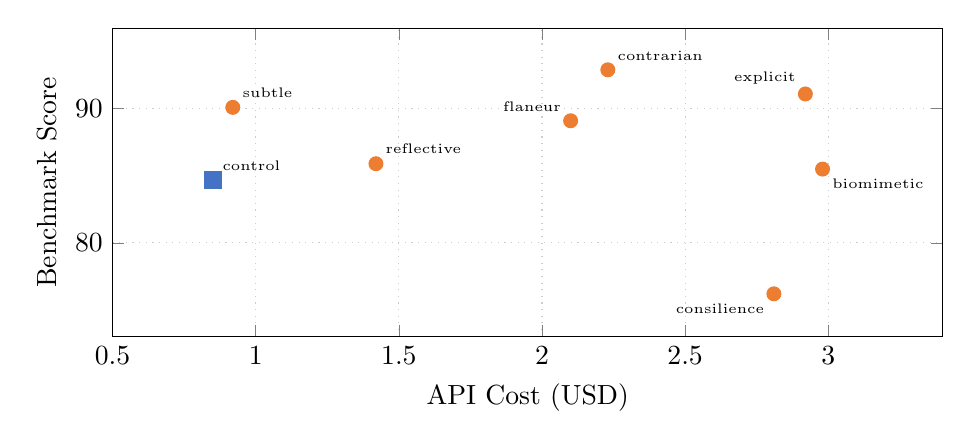
\begin{tikzpicture}
\begin{axis}[
    width=\textwidth,
    height=5.5cm,
    xlabel={API Cost (USD)},
    ylabel={Benchmark Score},
    xmin=0.5, xmax=3.4,
    ymin=73, ymax=96,
    grid=major,
    grid style={dotted,gray!40},
    only marks,
    mark size=2.5pt,
]
% Control point (blue square)
\addplot[controlblue, mark=square*, mark size=3pt]
  coordinates {(0.85,84.7)};
% Wiki points (orange circles)
\addplot[wikiorange, mark=*, mark size=2.5pt]
  coordinates {
    (0.92,90.1)
    (2.92,91.1)
    (1.42,85.9)
    (2.10,89.1)
    (2.81,76.2)
    (2.98,85.5)
    (2.23,92.9)
  };
% Labels
\node[font=\tiny, anchor=south west] at (axis cs:0.85,84.7) {control};
\node[font=\tiny, anchor=south west] at (axis cs:0.92,90.1) {subtle};
\node[font=\tiny, anchor=south east] at (axis cs:2.92,91.1) {explicit};
\node[font=\tiny, anchor=south west] at (axis cs:1.42,85.9) {reflective};
\node[font=\tiny, anchor=south east] at (axis cs:2.10,89.1) {flaneur};
\node[font=\tiny, anchor=north east] at (axis cs:2.81,76.2) {consilience};
\node[font=\tiny, anchor=north west] at (axis cs:2.98,85.5) {biomimetic};
\node[font=\tiny, anchor=south west] at (axis cs:2.23,92.9) {contrarian};
\end{axis}
\end{tikzpicture}
\subcaption{Benchmark score vs.\ API cost.  Control (blue square) is the
most cost-efficient; contrarian delivers the best score at 2.6$\times$ cost.}
\label{fig:cost}
\end{minipage}%
\hfill%
\begin{minipage}[t]{0.48\textwidth}
\centering
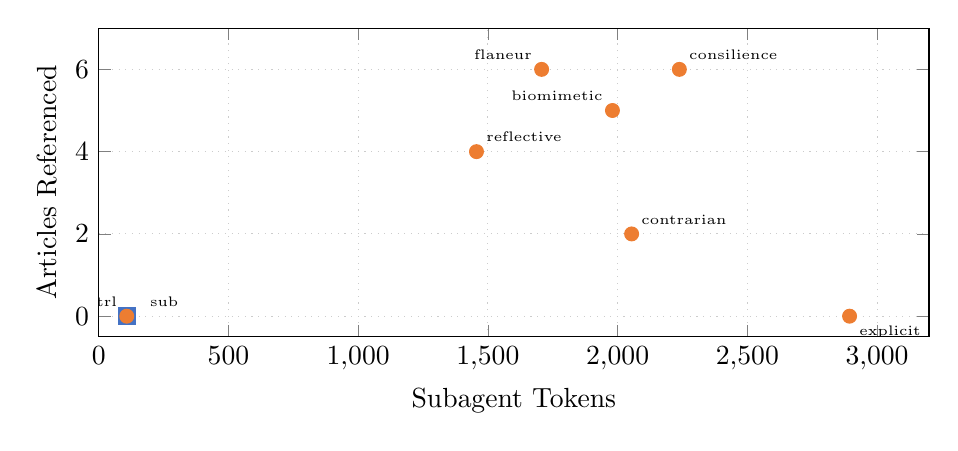
\begin{tikzpicture}
\begin{axis}[
    width=\textwidth,
    height=5.5cm,
    xlabel={Subagent Tokens},
    ylabel={Articles Referenced},
    xmin=0, xmax=3200,
    ymin=-0.5, ymax=7,
    grid=major,
    grid style={dotted,gray!40},
    only marks,
    mark size=2.5pt,
]
% Points
\addplot[controlblue, mark=square*, mark size=3pt]
  coordinates {(108,0)};
\addplot[wikiorange, mark=*, mark size=2.5pt]
  coordinates {
    (108,0)
    (2894,0)
    (1456,4)
    (1707,6)
    (2238,6)
    (1980,5)
    (2054,2)
  };
% Labels
\node[font=\tiny, anchor=south east] at (axis cs:108,0) {ctrl};
\node[font=\tiny, anchor=south west] at (axis cs:160,0) {sub};
\node[font=\tiny, anchor=north west] at (axis cs:2894,0) {explicit};
\node[font=\tiny, anchor=south west] at (axis cs:1456,4) {reflective};
\node[font=\tiny, anchor=south east] at (axis cs:1707,6) {flaneur};
\node[font=\tiny, anchor=south west] at (axis cs:2238,6) {consilience};
\node[font=\tiny, anchor=south east] at (axis cs:1980,5) {biomimetic};
\node[font=\tiny, anchor=south west] at (axis cs:2054,2) {contrarian};
\end{axis}
\end{tikzpicture}
\subcaption{Research effort vs.\ knowledge extraction.  Explicit researched
the most but extracted nothing; contrarian extracted high-impact insights.}
\label{fig:wiki}
\end{minipage}
\caption{Cost--performance trade-off (left) and Wikipedia research
patterns (right).}
\label{fig:scatters}
\end{figure*}

\FloatBarrier

% ─────────────────────────────────────────────────────────
% 4. WHAT EACH AGENT BUILT
% ─────────────────────────────────────────────────────────
\section{What Each Agent Built}

Table~\ref{tab:arch} summarizes the architectural choices made by each
condition.  Despite identical problem specifications, the eight agents
produced strikingly different designs.

\begin{table*}[t]
\centering\small
\caption{Architectural comparison across conditions.  WLC = weighted
least-connections; WRR = weighted round-robin; CB = circuit breaker;
EWMA = exponential weighted moving average; AIMD = additive increase /
multiplicative decrease; ACO = ant colony optimization; Po2RC = power-of-two
random choices.}
\label{tab:arch}
\begin{tabular}{@{}lllllr@{}}
\toprule
\textbf{Condition} & \textbf{Routing} & \textbf{Health Tracking}
  & \textbf{Shedding} & \textbf{Recovery} & \textbf{LOC} \\
\midrule
control     & WLC          & EWMA + sliding window
  & Fixed thresholds       & Quadratic ramp     & 471 \\
explicit    & CB states    & EWMA + circuit breaker
  & Hysteresis (70/80\%)   & AIMD               & 534 \\
subtle      & WLC          & Dual-EMA
  & Fixed thresholds       & Fast weight ramp   & 378 \\
reflective  & WLC          & Composite score + CB
  & AIMD thresholds        & AIMD               & 466 \\
flaneur     & WRR          & Geometric mean (3 axes)
  & Hysteresis + 4-state   & State machine      & 548 \\
consilience & Two-level    & Sigmoid from latency
  & Staged + UFLS          & Asymmetric 6:1     & 531 \\
biomimetic  & ACO pheromone & Baroreceptor sensing
  & ISR-like progressive   & Pheromone rebuild  & 444 \\
contrarian  & Po2RC        & Asymmetric EWMA
  & Proportional admission & Adaptive ramp      & 539 \\
\bottomrule
\end{tabular}
\end{table*}

\textbf{Control} (471~LOC) implements weighted least-connections routing
with EWMA latency and sliding-window success rate.  Priority-based
shedding activates at fixed capacity thresholds.  A solid, no-frills
baseline.

\textbf{Explicit} (534~LOC) builds a three-state circuit breaker
(CLOSED/OPEN/HALF\_OPEN) with AIMD capacity management borrowed from TCP
congestion control.  Hysteresis on shedding thresholds (enter at 70\%,
exit at 80\%) prevents oscillation---a structural advantage the judge
highlighted.

\textbf{Subtle} (378~LOC) is the leanest implementation.  Architecturally
near-identical to control, it never discovered the Wikipedia tools.  Yet
it benchmarks 3rd, suggesting the contract-based specification alone
improved code quality.

\textbf{Reflective} (466~LOC) overlays a circuit breaker on weighted
least-connections, citing the 2003 Northeast blackout and Gmail 2012
outage.  Conservative and well-proportioned---the ``measure twice''
approach.

\textbf{Flaneur} (548~LOC) uses weighted round-robin with three
independent health axes (latency, error rate, probe latency) combined via
geometric mean.  Inspired by monocoque structures from a random Wikipedia
walk, its four-state machine includes explicit hysteresis.

\textbf{Consilience} (531~LOC) is the most ambitious: two-level shedding
with per-backend stage gating and system-level UFLS (from power grid
engineering), sigmoid health scoring, and six cross-domain references.
The most sophisticated architecture---and the worst benchmark score.

\textbf{Biomimetic} (444~LOC) implements pheromone-weighted ACO routing
with 10\% random exploration.  Baroreceptor sensing (latency derivative)
provides predictive detection.  The most biologically faithful
implementation excels at asymmetric backends (0.98) but introduces
variance that hurts steady-state~(0.68).

\textbf{Contrarian} (539~LOC) uses power-of-two-random-choices routing
(pick two candidates, route to the better one).  Asymmetric EWMA---fast
degrade ($\alpha{=}0.4$), slow recover ($\alpha{=}0.08$)---prevents
detection lag.  Proportional admission replaces cliff-based shedding.
The adversarial research strategy produced the highest benchmark score.

% ─────────────────────────────────────────────────────────
% 5. DISCUSSION
% ─────────────────────────────────────────────────────────
\section{Discussion}

Six conclusions emerge from this experiment.

\textbf{1.\ Adversarial research produces the most robust code.}
Contrarian actively searched for what could go wrong before coding.  This
led to the discovery of the recovery deadlock bug (stale data deque with
zero-weight backends), which it avoided and control did not.  The result
was the highest benchmark score (92.9) and the largest judge margin
($+20$).

\textbf{2.\ Architectural ambition can hurt.}  Consilience built the most
sophisticated architecture (two-level shedding, sigmoid health, six
cross-domain references) but scored last on benchmarks (76.2).  Its
degradation detection scored 0.18---a basic scenario that six other
conditions handled adequately.  Sophistication is not a proxy for
correctness.

\textbf{3.\ The judge and benchmark measure different things.}  The judge
evaluates architecture, novelty, and cross-domain insight.  The benchmark
evaluates whether the code actually works under fault injection.  Both are
needed: the judge alone would rank consilience 1st; the benchmark alone
would miss biomimetic's creative value.  For production evaluation,
behavioral benchmarks should take precedence.

\textbf{4.\ Subtle is surprisingly competitive.}  Despite barely using
Wikipedia (108 subagent tokens, zero articles), subtle benchmarks 3rd
(90.1).  This may indicate that the contract-based problem
specification---with its explicit interface, enumerated priorities, and
behavioral requirements---does more work than the Wikipedia access.

\textbf{5.\ Cost scales with research depth, not quality.}  Biomimetic
cost 3.5$\times$ control for $+0.8$ benchmark points.  Contrarian cost
2.6$\times$ for $+8.2$ points.  The correlation between cost and quality
is weak---the cheapest Wikipedia condition (subtle, \$0.92) outperforms
the most expensive (biomimetic, \$2.98) by 4.6 points.

\textbf{6.\ Creative approaches trade consistency for adaptiveness.}
Biomimetic's ACO routing excels at asymmetric backends (0.98) but
introduces variance that hurts steady-state (0.68) and flapping resistance
(0.73).  Standard approaches are more predictable; novel algorithms
require broader scenario coverage to validate.

\paragraph{Limitations.}
This is a single-problem ($N{=}1$), single-model (Claude), single-judge
experiment.  The results may not generalize to other problem types,
models, or evaluation approaches.  Each condition was run once, so we
cannot estimate within-condition variance.  The LLM judge's scores vary
across comparisons (control scored between 52 and 63 across seven
pairings), introducing noise in the margin estimates.

% ─────────────────────────────────────────────────────────
% 6. CONCLUSION
% ─────────────────────────────────────────────────────────
\enlargethispage{2\baselineskip}
\section{Conclusion}

Wikipedia access can improve LLM-generated code, but the research
strategy matters more than the access itself.  Adversarial research
(contrarian) produced the most robust implementation by finding failure
modes before they became bugs.  Undirected or overly ambitious research
strategies yielded diminishing or negative returns.  Evaluating generated
code requires multiple complementary methods---design-quality judges and
behavioral benchmarks capture different dimensions of quality and can
disagree sharply on the same implementation.

\end{document}
